\section{Auswertung}

\subsection{Messungen bis 1 Bar}

\subsubsection{Plot der Messwerte und Funktionen}
\begin{figure}[htp]
    \centering
    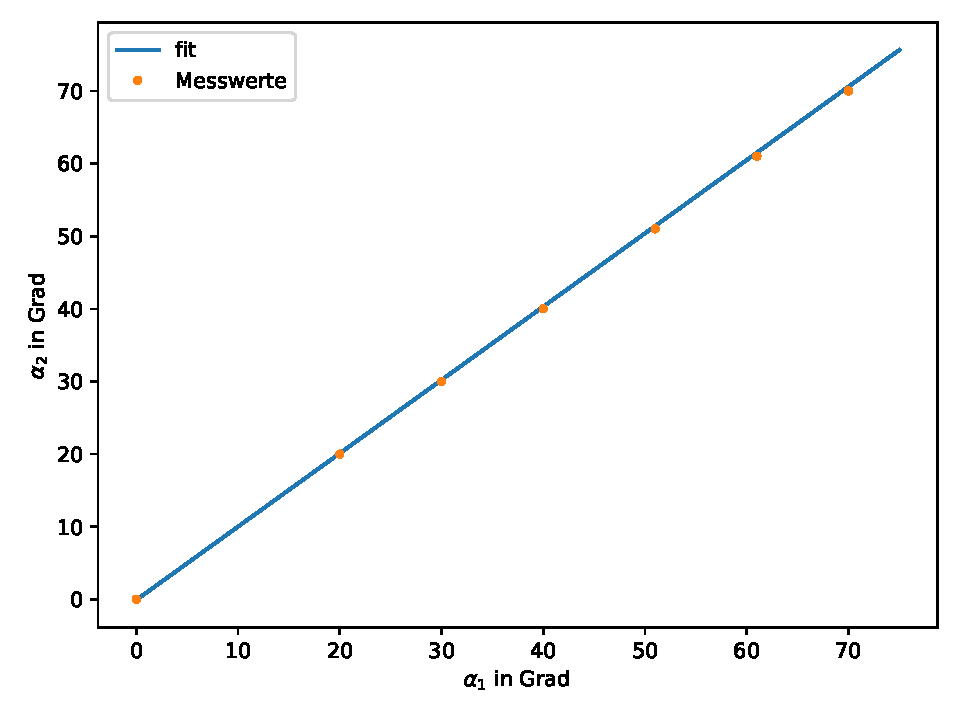
\includegraphics[width=0.7\textwidth]{build/plot1.pdf}
    \caption{Ein Plot der Messwerte inklusive der gefiteten Funktionen.}
    \label{img:plot1}
\end{figure}
\FloatBarrier

\subsubsection{Berechnung von L}

Die gefittete Funktion auf die Messwerte \ref{tab:messung1} wurde mithilfe einer linearen Regression berechnet.
Die Rechnung führt zu der Formel:
\begin{align}
    y&=m\cdot x+n \nonumber\\
    \implies y&=-4372.84836719 \cdot x+29.98959435 \nonumber
\end{align}
Mit Hilfe der Gaskonstante $\symup{R}$   \footnote{Quelle: \url{https://www.chemie.de/lexikon/Universelle_Gaskonstante.html}(Besucht am 09.11.2020)}
und der Steigung der Ausgleichsgerade lässt sich nun eine gute Näherung für $L$, für Werte kleiner als $\SI{1}{\bar}$ berechnen.
Die $-1$ rührt dabei daher, dass $L$ aus einer negativen Steigung hergeleitet wird, aber nur ihr Betrag relevant ist.
\begin{align}
    L&=(-1) \cdot m \cdot \symup{R} \nonumber\\
    \implies L&\approx\SI{36.3578843(6667737)e3}{\joule\per\mol} \nonumber
\end{align}\\
Anschließend soll die innere Verdampfungswärme $L_i$, pro Molekül, bestimmt werden.\\
Dies geschieht über das berechnen der äußeren Verdampfungswärme $L_a$, um $L_i$ aus der Formel $L=L_i+L_a$ zu bestimmen.\\
Die äußere Verdampfungswärme ist dabei die Energie, die nötig ist um das Volumen eines Stoffes von $V_F$ auf $V_D$ auszudehnen,
also die Volumenarbeit $W=pV$.\\
Wenn man nun als äußere Verdampfungswärme $T=373 \si{\kelvin}$ also $T\approx 100 \si{\celsius}$ annimmt lässt sich über die Allgemeine Gasgleichung $L_i$ bestimmen.
\begin{equation}
    L_a=pV=\symup{R} \cdot T = \SI{3101.2946}{\joule\per\mol} \nonumber
\end{equation}
Daraus folgt dann:
\begin{align}
    L_i&=L-L_a \nonumber\\
    L_i&=\SI{33.2565897(6667737)e3}{\joule\per\mol} \nonumber
\end{align}
Um dies dann pro Molekül zu betrachten wird der Wert durch die Avogadro-Konstante $\symup{N_A}$\footnote{Quelle: \url{https://www.chemie.de/lexikon/Avogadro-Konstante.html}(Besucht am 15.11.2020)}
geteilt und zusätzlich, für bessere Anschaulichkeit,
noch in $\si{\electronvolt}$ umgerechnet.
\begin{equation}
    L_i=\SI{34.47(69)e-2}{\electronvolt} \nonumber
\end{equation}

\clearpage


\subsubsection{Die Messwerte bis 1 Bar}

\begin{table}[H]
    \centering
    %\caption{Die Messwerte}
    \begin{tabular}{ S [table-format=4.0] S [table-format=3.0]}
        \toprule
        {$P \mathbin{/} \si{\milli\bar}$} & {$T \mathbin{/} \si{\celsius}$}\\
        \midrule
        30 & 22 \\
        50 & 26\\
        108 & 40\\
        153 & 51\\
        200 & 58\\
        250 & 64\\
        300 & 69\\
        350 & 73\\
        400 & 76\\
        450 & 79\\
        500 & 83\\
        550 & 86\\
        600 & 88\\
        650 & 91\\
        700 & 94\\
        750 & 97\\
        800 & 98\\
        850 & 100\\
        900 & 102\\
        950 & 104\\
        1000 & 108\\
        \bottomrule
    \end{tabular}
\caption{Eine Tabelle der Messwerte bis $\SI{1000}{\milli\bar}$.%wobei die Temperaturen mit einem Fehler von  $\increment T = \SI{0.1}{\celsius}$ behaftet sind.
}
\label{tab:messung1}
\end{table}












%nervige formel






\subsection{Messung bis 15 Bar}


\subsubsection{Bestimmung einer Funktion L(T)}


Um eine Funktion $L(T)$ zu bestimmen benötigen wir erst einen Fit $p(T)$ auf die Messreihe \ref{tab:messung2}, um später
$p$ und $\frac{\symup{d}p}{\symup{d}t}$, in , approximieren zu können.\\
Zunächst nehmen wir aber die Clausius-Clapeyronsche Gleichung \refeq{eqn:sum} und stellen sie nach der Verdampfungswärme $L$ um.
\begin{equation}
    L= T \cdot (V_\text{D}-V_\text{F}) \frac{\symup{d}p}{\symup{d}T}
    \label{eqn:clausL}
\end{equation}
Da bei disem Experiment ein Sättigunsdampdruck erreicht wird, welcher nicht vom Volumen abhängig ist lässt sich $V_D$ nicht mehr 
über die Allgemeine Gasgleichung bestimmen. Stattdessen nutzen wir die Näherung :
\begin{align}
   \symup{R}\cdot T &= \left( p + \frac{A}{V_D^2}\right)\cdot V_D  &
    &\text{mit} &
    A&=\SI{0.9}{\joule\cubic\metre\per\mol\squared} \nonumber \\
    \implies V_D&=\frac{\symup{R}\cdot T}{2p} \pm \sqrt{\frac{\symup{R}^2\cdot T^2}{4p^2}-\frac{A}{p}} \nonumber
    \intertext{Da man $V_F$ vernachlässigen kann gilt für die Gleichung \refeq{eqn:clausL} $(V_\text{D}-V_\text{F}) \approx V_D$.
    Einsetzen führt dann zu:}
    L&=T\left(\frac{\symup{d}p}{\symup{d}t}\frac{\symup{R}\cdot T}{2p} \pm\sqrt{\frac{\symup{R}^2\cdot T^2}{4p^2}-\frac{A}{p}}\right)\frac{\symup{d}p}{\symup{d}t} \nonumber\\
    L&=\frac{T}{p}\left( \frac{\symup{R} \cdot T}{2p} \pm\sqrt{\frac{\symup{R}^2\cdot T^2}{4p^2}-\frac{A}{p}} \right)\frac{\symup{d}p}{\symup{d}t} \label{eqn:ohnedp}
    \intertext{Um $\frac{\symup{d}p}{\symup{d}t}$ in \refeq{eqn:ohnedp} zu approximieren bestimmen wir, wie zuvor erläutert, eine Fit-Funktion 3.Grades
    für die Temperatur $T$ und den Druck $p$ und differenzieren sie anschließend.}  \nonumber
\end{align}
Der Fit auf $p$ und seine dazugehörige Ableitung sind: 
\begin{align}
    p(T)&=a\cdot T^3+b\cdot T^2 + c\cdot T+d \nonumber\\
    \frac{\symup{d}p}{\symup{d}t}&=3a\cdot T^2+2b\cdot T + c \nonumber
\end{align}
Mit den Werten 
\begin{table}[H]
    \centering
    \sisetup{table-format=1.3}
    \begin{tabular}{ S S [table-format=3.5] @{$ \pm{}$} S [table-format=3.5] S }
        \toprule
        {Parameter} & \multicolumn{3}{c}{ Bestimmte Werte} \\
        \midrule
        \text{a}	&\num{9.29297e-06}  & \num{1.97123e-06} & \; \si{\pascal\per\cubic\kelvin}\\
        \text{b}	&\num{-0.01029}  & \num{0.00256} & \; \si{\pascal\per\kelvin\squared}\\
        \text{c}	&\num{3.84663}  & \num{1.10409} & \; \si{\pascal\per\kelvin}\\
        \text{d}	&\num{-485.74494}  & \num{158.58876} & \; \si{\pascal}\\
        \bottomrule
        \\
    \end{tabular}
\caption {Berechnete Werte für die Polynome der Fit-Funktion gerundet auf die fünfte Nachkommastelle.}
\label{tab:params}
\end{table}

\begin{figure}[H]
    \centering
    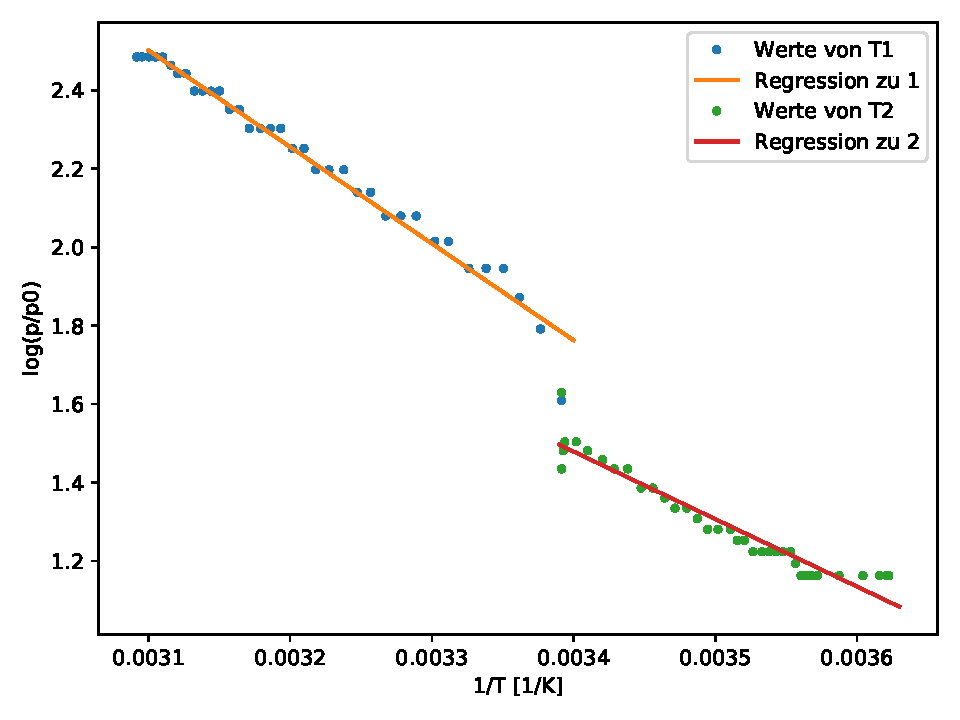
\includegraphics[width=0.7\textwidth]{build/plot2.pdf}
    \caption{Die Messwerte inklusive der Fit-Funktion.}
    \label{img:plot1}
\end{figure}


Einsetzen der Fit-Funktionen in \refeq{eqn:ohnedp} führt zu:
\begin{equation}
    L(T)=\left( \frac{\symup{R} \cdot T}{2p} \pm\sqrt{\frac{\symup{R}^2\cdot T^2}{4p^2}-\frac{A}{p}} \right)\frac{3a\cdot T^3+2b\cdot T^2 + c\cdot T}{a\cdot T^3+b\cdot T^2 + c\cdot T+d}
    \label{eqn:mitdp}
\end{equation}
Durch das $\pm$ erhalte ich zwei Funktionen für die Verdampfungswärme. Durch einsetzen von beliebigen Zahlen sieht man, dass die Funktion
für das Minus \ref{img:minus} negative Werte liefert, weswegen sie keine sinnvolle Lösung bietet.\\
Die Funktion \ref{img:plus} für das Plus hingegen, liefert jedoch eine streng mnoton fallende Funktion für $L$.
Dies ergibt auch Sinn, da die Verdampfungswäme immer weiter abnehmen sollte, je näher man der kritischen Temperatur kommt, bei der $L=0$ gilt.

\subsubsection{Plots der Funktionen der Verdampfungswärme}
\FloatBarrier
\begin{figure}[H]
    \centering
    \includegraphics[width=0.7\textwidth]{build/plot3+.pdf}
    \caption{Ein Plot der Funktion $L_+(T)$.}
    \label{img:plus}
\end{figure}

\begin{figure}[H]
    \centering
    \includegraphics[width=0.7\textwidth]{build/plot3-.pdf}
    \caption{Ein Plot der Funktion $L_-(T)$.}
    \label{img:minus}
\end{figure}

\FloatBarrier







\subsubsection{Die Messwerte bis 15 Bar}

\begin{table}[H]
    \centering
    %\caption{Die Messwerte}
    \begin{tabular}{ S [table-format=3.0] S [table-format=3.0]}
        \toprule
        {$P \mathbin{/} \si{\bar}$} & {$T \mathbin{/} \si{\celsius}$}\\
        \midrule
        1 & 118.0\\
        2 & 129.5\\
        3 & 141.0\\
        4 & 150.0\\
        5 & 157.0\\
        6 & 163.5\\
        7 & 168.0\\
        8 & 172.5\\
        9 & 177.0\\
        10 & 181.5\\
        11 & 185.5\\
        12 & 189.0\\
        13 & 192.0\\
        14 & 195.0\\
        15 & 198.5\\
        \bottomrule
    \end{tabular}
\caption{Eine Tabelle der Messwerte bis $\SI{15}{\bar}$.%wobei die Temperaturen mit einem Fehler von  $\increment T = \SI{0.1}{\celsius}$ behaftet sind.
}
\label{tab:messung2}
\end{table}


